\documentclass{llncs}
\usepackage{makeidx}
\usepackage{enumerate}
\usepackage[dvips]{graphicx}
\usepackage{subfigure}
\usepackage{authblk}
\usepackage{amssymb}
\usepackage{amsmath}
\usepackage{amsfonts}
\usepackage{booktabs}
\usepackage{threeparttable}
\usepackage{algorithm}
\usepackage{algorithmicx}
\usepackage{algpseudocode}
\usepackage{textcomp}
\renewcommand{\algorithmicrequire}{\textbf{Input}}
\renewcommand{\algorithmicensure}{\textbf{Output}}
\makeatletter 
  \newcommand\figcaption{\def\@captype{figure}\caption} 
  \newcommand\tabcaption{\def\@captype{table}\caption} 
  \newcommand{\tabincell}[2]{\begin{tabular}{@{}#1@{}}#2\end{tabular}}
\makeatother
% \usepackage{fancyhdr}
% \pagestyle{fancy}
% \fancyhf{}
% \renewcommand{\headrulewidth}{0pt}
% \renewcommand{\footrulewidth}{0pt}
% \fancyhead[RO]{{\scriptsize Extended Refined Ordering Relations with Uncertainty \qquad\thepage}}
% \fancyhead[LE]{{\scriptsize \thepage\qquad Shuhao Wang, Lijie Wen, Zixuan Wang, Jianmin Wang and Jianwen Su}}
\begin{document}
\frontmatter 
\pagestyle{headings}
\addtocmark{Extended Refined Ordering Relations with Uncertainty}

\mainmatter
\title{A Behavioral Similarity Measure for Process Models based on Extended Refined Ordering Relations with Uncertainty}
\titlerunning{Extended Refined Ordering Relations with Uncertainty}

\author[$\$$]{Shuhao Wang}
\author[$\$$]{Lijie Wen}
\author[$\$$]{Zixuan Wang}
\author[$\$$]{Jianmin Wang}
\author[$\#$]{Jianwen Su}
\authorrunning{Shuhao Wang et al.}
\tocauthor{Shuhao Wang, Lijie Wen, Zixuan Wang, Jianmin Wang and Jianwen Su}
\affil[$\$$]{School of Software, Tsinghua University, Beijing 100084, P.R. China \authorcr
\texttt{shudiwsh2009@gmail.com,wenlj@tsinghua.edu.cn,
iamwangzixuan@hotmail.com,jimwang@tsinghua.edu.cn}}
\affil[$\#$]{Department of Computer Science, UC Santa Barbara, USA \authorcr
\texttt{su@cs.ucsb.edu}}
\institute{}

\maketitle

\begin{abstract}
Tao Jin has proposed new ordering relations between execution of tasks in business process models. He also gave an algorithm to compute the refined ordering relations for acyclic process models based on unfolding technology. However, his algorithm cannot work well for cyclic WF-nets and process models with invisible tasks. We extend his work and present a refinement of the relations. To better measure the differentiation between process models, we introduce the notion of sequential direct adjacency. Also, we propose an algorithm to compute relations in arbitrary WF-nets and utilize them to measure the similarity between process models.
\keywords{Business Process Model, Refined Ordering Relations with Uncertainty, Sequential Direct Adjacency, Behavioral Similarity}
\end{abstract}

\section{Introduction}\label{sec:introduction}

In a seminal paper \cite{jin2014computing}, Tao Jin has proposed new ordering relations between execution of tasks in business process models. He refines the causal and concurrency relations between two events in a concurrent system with uncertainty according to whether one task is always executed with the other task in the same instance. He then proposes some rules for adjacent tasks and some transitive laws for nonadjacent tasks, based on which he proposes an algorithm to compute the refined ordering relations for acyclic process models. The algorithm is done on the unfolding of a WF-net \cite{mcmillan1995technique,esparza1996improvement}.

Although Tao Jin' work is elegant, it has some drawbacks. First of all, for cyclic Petri nets, his algorithm cannot work well. According to his paper, the problem arises from the Global Fairness Assumption \cite{kindler1999liveness}. Secondly, invisible tasks have not been taken into consideration so that two models with different behavioral semantics may have the same set of ordering relations. To solve these problems, we extend his ordering relations to more trivial cases which is inspired by the work of DecSerFlow \cite{van2006decserflow}, and introduce the concept of sequential direct adjacency to better differentiate the behavioral semantics of two process models. Of course, we propose an algorithm to compute our relations in arbitrary WF-nets.

Furthermore, since our refined relations have a strong ability to represent the behavioral semantics of a process model and can efficiently measure the tiny differentiation between two models, even when they contain invisible tasks, we utilize them as a proper metric to measure the similarity between two process models.

Similarity measure can be widely used in many scenarios, such as model retrieval, process mining and model classification. There have been various proposals to this topic: based on textual information, the structure of process models, and their execution semantics \cite{kunze2011behavioral}.
% TODO: mainstream algorithms

In this paper, we propose a behavioral similarity measure based on the extended refined ordering relations with uncertainty. It satisfies metric properties, especially the triangle inequality \cite{zezula2006similarity}. The algorithm firstly extracts three types of relations and generates the relation sets of a process model. By measuring the similarity between relation sets of process models, a similarity value is finally given by the algorithm. We conduct experiments using process models from real enterprises and the results show that our similarity measure is both efficient and effective.

The remainder of this paper is structured as follows: The next section gives formal preliminaries that will be used in this paper. The concept and computation of extended refined ordering relations as well as sequential direct adjacency are introduced in Section \ref{sec:relations}. We present the method to measure process model similarity in Section \ref{sec:similarity}. Section \ref{sec:experiments} shows the results of an experimental evaluation, before we conclude the paper and give an outlook on future work in Section \ref{sec:conclusion}.

\section{Preliminaries}\label{sec:preliminaries}
Our work is to measure the similarity between two process models. There are many different notations to describe the business process, such as Business Process Model and Notation (BPMN), Event-driven Process Chain (EPC), Yet Another Workflow Language (YAWL) and Petri Net Markup Language (PNML). Since Petri net is suitable to analyze the behavior of process models, we will show our algorithm on Petri net. The concept of the Petri net has its origin in Carl Adam Petri's dissertation \cite{petri1966kommunikation}.

\begin{definition}[Petri net]\label{def:petrinet}
A Petri net is a triple $(P,T,F)$:
	\begin{itemize}
		\item[-] $P$ is a finite set of places;
		\item[-] $T$ is a finite set of transitions ($P\cap T=\emptyset$);
		\item[-] $F\subseteq(P\times T)\cup(T\times P)$ is a set of arcs (flow relation).
	\end{itemize}
\end{definition}

For more details about Petri net, please refer to the work of Murata \cite{murata1989petri}. A Petri net which models a workflow process definition is called a WorkFlow net (WF-net) \cite{van1998application}.

\begin{definition}[WF-net]\label{def:wfnet}
A Petri net $PN=(P,T,F)$ is a WF-net (Workflow net) if and only if:
	\begin{itemize}
		\item[-] $PN$ has two special places: $i$ and $o$. Place $i$ is a source place: $\bullet i=\emptyset$. Place $o$ is a sink place: $o\bullet =\emptyset$;
		\item[-] If we add a transition $t^{*}$ to $PN$ which connects place $o$ with $i$ (i.e. $\bullet t^{*}=\{o\}$ and $t^{*}\bullet=\{i\}$), then the resulting Petri net is strongly connected.
	\end{itemize}
\end{definition}

We extract the relations between activities on a WF-net. A intuitive idea is to generate the reachability graph of a model. We need to consider all possible interleavings of concurrent events, which causes the state explosion problem in a concurrent system \cite{mcmillan1995technique}. Javier Esparza proposed the notion of complete prefix unfolding to avoid this \cite{esparza1996improvement}, based on the improvement of McMillan's unfolding algorithm \cite{mcmillan1995technique}. Therefore, we use his work instead.

\begin{definition}[Ordering Relations]\label{def:orderingRelations}
There are three types of ordering relations between nodes of a net,
	\begin{itemize}
		\item[-] two nodes $x$ and $y$ are in causal relation, denoted by $x<y$, if the net contains a path with at least one arc leading from $x$ to $y$;
		\item[-] $x$ and $y$ are in conflict relation, denoted by $x\#y$, if the net contains two paths $st_{1}...x_{1}$ and $st_{2}...x_{2}$ starting at the same place $s$, and such that $t_{1}\neq t_{2}$;
		\item[-] $x$ and $y$ are in concurrency relation, denoted by $x~co~y$, if neither $x<y$ nor $y<x$ nor $x\#y$.
	\end{itemize}
\end{definition}

\begin{definition}[Occurrence net]\label{def:occurrenceNet}
An occurrence net is a Petri net $O=(B,E,A)$ such that $\forall x,y\in B\cup E:(x,y)
\in A^{+}\Rightarrow(y,x)\notin A^{+}$ and $\forall b\in B:|\bullet b|\leq 1$.
\end{definition}

\begin{definition}[Branching process]\label{def:branchingProcess}
A branching process of a Petri net system $\Sigma=(P,T,F,M_{0})$ is a labelled occurrence net $\beta=(B,E,A,f)$ where the labelling function $f$ satisfies the following properties:
	\begin{itemize}
		\item[-] $f(B)\subseteq P$ and $f(E\subseteq T$ ($f$ preserves the nature of nodes);
		\item[-] for every $e\in E$, the restriction of $f$ to $\bullet e$ is a bijection between $\bullet e$ (in $\Sigma$) and $\bullet f(e)$ (in $\beta$), and similarly for $e\bullet$ and $f(e)\bullet$ ($f$ preserves the environments of transitions);
		\item[-] the restriction of $f$ to $Min(O)$ is bijection between $Min(O)$ and $M_{0}$ ($\beta$ "starts" at $M_{0}$), where $Min(O)$ denotes the set of minimal elements of $B\cup E$ with respect to the causal relation;
		\item[-] for every $e_{1},e_{2}\in E$, if $\bullet e_{1}=\bullet e_{2}$ and $f(e_{1})=f(e_{2})$ then $e_{1}=e_{2}$ ($\beta$ does not duplicate the transitions of $\Sigma$).
	\end{itemize}
\end{definition}

A Petri net system has infinite branching processes, which differ on "how much it unfolds". The complete finite prefix is the minimal one which contains all the markings contained in the branching process.

\begin{definition}[Complete Prefix Unfolding]\label{def:cpu}
Let $\beta=(B,E,A,f)$ be a branching process of a Petri net system $\Sigma=(P,T,F,M_{0})$, every condition $b\in B$ has a corresponding place $p\in P$ and every event $e\in E$ has a corresponding transition $t\in T$.
	\begin{itemize}
		\item[-] A local configuration $\lceil e\rceil$ of a event $e$ in an occurrence net is the set of events that precede $e$.
		\item[-] The final marking of a local configuration $Mark(\lceil e\rceil)$ is the set of conditions that are marked after all the events in $\lceil e\rceil$ fire.
		\item[-] An adequate order $\prec$ is a strict well-founded partial order on local configurations, so that $\lceil e\rceil\subset\lceil e'\rceil$ implies $\lceil e\rceil\prec\lceil e'\rceil$.
		\item[-] An event $e$ of a branching process is a cutoff event if there exists a corresponding event $e'$, such that $Mark(\lceil e\rceil)=Mark(\lceil e'\rceil)$ and $\lceil e\rceil\prec\lceil e'\rceil$.
		\item[-] A complete prefix unfolding is the greatest backward closed subnet of an occurrence net containing no events after cutoff events.
	\end{itemize}
\end{definition}

Definitions about complete prefix unfolding and related concepts come from the work of Esparza \cite{esparza1996improvement} and Polyvyanyy \cite{polyvyanyy2010structuring}.

\begin{figure}[htbp]
\centering
\subfigure[] {
	\begin{minipage}[b]{0.7\textwidth}
		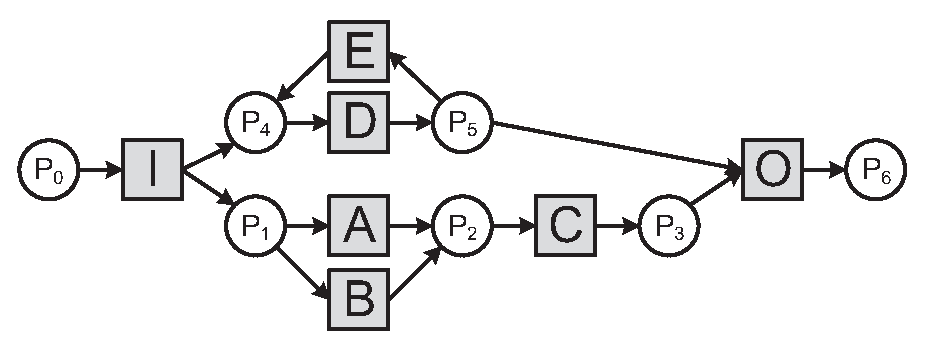
\includegraphics[width=1\textwidth]{fig_example_petri.eps}
		\label{fig:examplePetri}
	\end{minipage}
}
\subfigure[] {
	\begin{minipage}[b]{0.7\textwidth}
		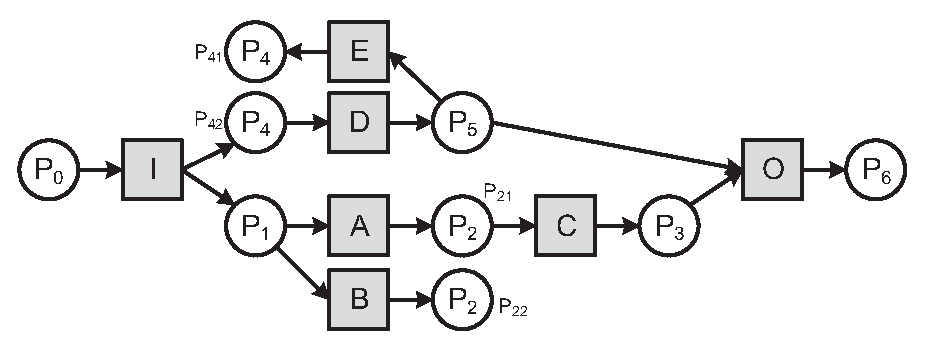
\includegraphics[width=1\textwidth]{fig_example_cpu.eps}
		\label{fig:exampleCpu}
	\end{minipage}
}
\caption{A sound WF-net example and its complete prefix unfolding}
\label{fig:examplePetriAndCpu}
\end{figure}

\begin{example}\label{ex:petriAndCpu}
Fig. \ref{fig:examplePetriAndCpu} shows a sound WF-net and its complete prefix unfolding. In the unfolding in Fig. \ref{fig:exampleCpu}, transitions labelled as $B$ and $E$ are cutoff transitions.
\end{example}

Our extended relations are inspired by the work in \cite{van2006decserflow}, which utilizes the relations between activities to model a process.
\begin{definition}[Relation Formulas]\label{def:relationFormulas}
Let $A$ and $B$ be two activities of a process, $A$ and $B$ are in the following relation formulas:\footnote{Note that the relation formulas are not complete here, since we only need part of them. For more details, please refer to the work of Alast \cite{van2006decserflow}.}
	\begin{itemize}
		\item[-] Alternate Response: after the execution of an activity $A$ activity $B$ has to be executed and between the execution of each two $A$ at least one activity $B$ has to be executed.
		\item[-] Alternate Precedence: every instance of activity $B$ has to be preceded by an instance of activity $A$ and the next instance of activity $B$ cannot be executed before the next instance of activity $A$ is executed.
	\end{itemize}
\end{definition}

\begin{example}\label{ex:relationFormulas}
In the model of Fig. \ref{fig:examplePetri}, transitions $D,E$ in the execution sequence $[I,D,E,D,E,D,E,O]$ satisfy the formula \textit{alternate response} and \textit{alternate precedence} while transitions $D,O$ do not satisfy the formula \textit{alternate response} and transitions $I,D$ do not satisfy the formula \textit{alternate precedence}.
\end{example}

\section{Extended Refined Ordering Relations with Uncertainty}\label{sec:relations}
In this section, we introduce the concept of extended refined ordering relations with uncertainty and its calculation from a WF-net. Let $\Sigma=(P,T,F,M_{0})$ be a sound WF-net, and $\beta=(B,E,A,f)$ be $\Sigma$'s complete prefix unfolding. Let $x,y\in E$ be events of the branching process.

It should be noticed that there would be cutoff events and cutoff conditions (conditions after those cutoff events) in the complete prefix unfolding of a WF-net. We can easily set a mapping between cutoff conditions and the conditions after the corresponding event of a cutoff event. Therefore, the path we defined above should not end on a cutoff condition, but will continue from the mapping of a cutoff condition to the end state instead. For example, in the complete prefix unfolding of Fig. \ref{fig:exampleCpu}, $[I,B]$ and $[I,D,E]$ are not paths, but $[I,B,C,O]$ and $[I,D,E,D,O]$ are paths.

\subsection{Extended Refined Causal and Inverse Causal Relations with Uncertainty}\label{subsec:causalAndInverseCausal}
A path means a directed path from the source condition to the end condition in the complete prefix unfolding. Let $S$ be the set containing all the paths of $\beta$, and $S_{x}$ be the set of the paths containing event $x$, i.e, $S_{x}=\{\rho\in S|x\in\rho\}$. Our extended causal and inverse causal relations are defined using the notion of $S_{x}$.

\begin{definition}[Always Causal]\label{def:alwaysCausal}
$x$ and $y$ are in always causal relation (denoted as $x\twoheadrightarrow y$) iff: $\forall\rho_{x}\in S_{x}$, $x$ and $y$ are in \textit{alternate response} relation, i.e., among all the paths containing event $x$, after the execution of every $x$ there must be at least one $y$ executed, and before that $y$ there cannot be another event $x$.
\end{definition}

\begin{definition}[Never Causal]\label{def:neverCausal}
$x$ and $y$ are in never causal relation (denoted as $x\nrightarrow y$) iff: $\forall\rho_{x}\in S_{x}$, there is no $y$ in $\rho_{x}$, or $x$ and $y$ are not in \textit{response} relation, i.e., among all the paths containing event $x$, after the execution of every $x$, there mustn't be an instance of $y$ executed.
\end{definition}

\begin{definition}[Sometimes Causal]\label{def:sometimesCausal}
$x$ and $y$ are in sometimes causal relation (denoted as $x\rightharpoonup y$) iff: $\forall\rho_{x}\in S_{x}$, $x$ and $y$ are neither in always causal relation nor in never causal relation.
\end{definition}

\begin{example}\label{ex:causalRelation}
In the model of Fig. \ref{fig:exampleCpu}, $A$ and $C$ are in \textit{always causal} relation ($A\twoheadrightarrow C$) since they are in \textit{alternate response} relation among all the paths containing $A$. $D$ and $O$ are in \textit{sometimes causal} relation ($D\rightharpoonup O$) since there may be another $D$ between the execution of the first $D$ and $O$, indicating that $D$ and $O$ are not in \textit{alternate response} relation. $C$ and $D$ are in \textit{never causal} relation ($C\nrightarrow D$).
\end{example}

\begin{definition}[Always Inverse Causal]\label{def:alwaysInverseCausal}
$x$ and $y$ are in always inverse causal relation (denoted as $y\twoheadrightarrow^{-1}x$) iff: $\forall\rho_{y}\in S_{y}$, $x$ and $y$ are in \textit{alternate precedence} relation, i.e., among all the paths containing event $y$, every instance of $y$ has to be preceded by an instance of $x$ and the next instance of event $y$ cannot be executed before the next instance of event $x$ is executed.
\end{definition}

\begin{definition}[Never Inverse Causal]\label{def:neverInverseCausal}
$x$ and $y$ are in never inverse causal relation (denoted as $y\nrightarrow^{-1}x$) iff: $\forall\rho_{y}\in S_{y}$, there is no $x$ in $\rho_{y}$, or $x$ and $y$ are not in \textit{precedence} relation, i.e., among all the paths containing event $y$, before the execution of every $y$, there mustn't be an instance of $a$ executed.
\end{definition}

\begin{definition}[Sometimes Inverse Causal]\label{def:sometimesInverseCausal}
$x$ and $y$ are in sometimes inverse causal relation (denoted as $y\rightharpoonup^{-1}x$) iff: $\forall\rho_{y}\in S_{y}$, $x$ and $y$ are neither in always inverse causal relation nor in never inverse causal relation.
\end{definition}

\begin{example}
In the model of Fig. \ref{fig:examplePetri}, $D$ and $O$ are in \textit{always inverse causal} relation ($O\twoheadrightarrow^{-1}D$) since they are in \textit{alternate precedence} relation among all the paths containing $O$. $A$ and $C$ are in \textit{sometimes inverse causal} relation ($C\rightharpoonup^{-1}A$) since there may be no instance of transition $A$ in some paths containing $C$ (such as $[I,B,C,O]$), indicating that $A$ and $C$ are not in \textit{precedence} relation. $C$ and $D$ are in \textit{never inverse causal} relation ($D\nrightarrow^{-1}C$).
\end{example}

We have identified several cases of causal and inverse causal relations and turn them into abstract formulas, as shown in Fig. \ref{fig:causalCases}. In thses cases, $A$ and $B$ are events of an unfolding. The edge labeled with "Loop $A$" means that there is a path starting from some node after $A$ and ending in some node before $A$ so that $A$ can be executed more than once. The edge labeled with "Skip $A$" means that there is a path starting from some node before $A$ and ending in some node after $A$ so that $A$ may not be executed. In other words, transitions inside a \textit{loop} structure can be executed more than once which transitions inside a \textit{skip} structure may not be executed.

\begin{figure}[htbp]
\centering
\subfigure[] {
	\begin{minipage}[b]{0.45\textwidth}
		\centering
		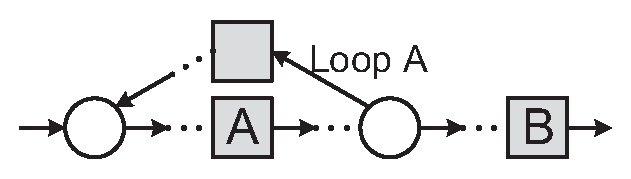
\includegraphics[width=0.6\textwidth]{fig_causal_case_a_1.eps}\\
		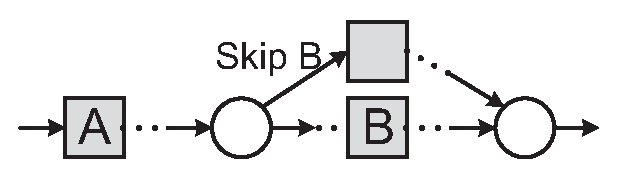
\includegraphics[width=0.6\textwidth]{fig_causal_case_a_2.eps}
	\end{minipage}
	\label{fig:causalCaseA}
}
\subfigure[] {
	\begin{minipage}[b]{0.45\textwidth}
		\centering
		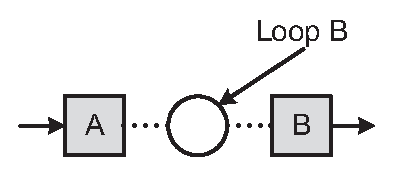
\includegraphics[width=0.6\textwidth]{fig_causal_case_b_1.eps}
		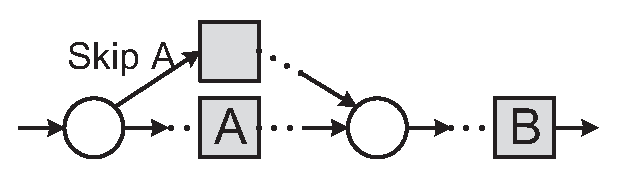
\includegraphics[width=0.6\textwidth]{fig_causal_case_b_2.eps}
	\end{minipage}
	\label{fig:causalCaseB}
}
\subfigure[] {
	\begin{minipage}[b]{0.45\textwidth}
		\centering
		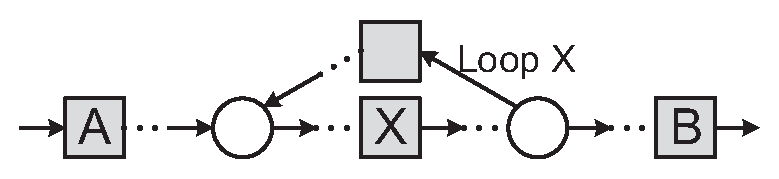
\includegraphics[width=0.8\textwidth]{fig_causal_case_c.eps}
	\end{minipage}
	\label{fig:causalCaseC}
}
\subfigure[] {
	\begin{minipage}[b]{0.45\textwidth}
		\centering
		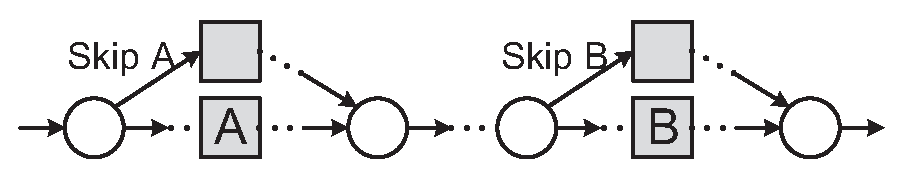
\includegraphics[width=0.8\textwidth]{fig_causal_case_d.eps}
	\end{minipage}
	\label{fig:causalCaseD}
}
\caption{Abstract formulas of causal and inverse causal relations. \subref{fig:causalCaseA} $A\rightharpoonup B, B\twoheadrightarrow^{-1}A$; \subref{fig:causalCaseB} $A\twoheadrightarrow B, B\rightharpoonup^{-1}A$; \subref{fig:causalCaseC} $A\twoheadrightarrow B, B\twoheadrightarrow^{-1}A$; \subref{fig:causalCaseD} $A\rightharpoonup B, B\rightharpoonup^{-1}A$.}
\label{fig:causalCases}
\end{figure}

For convenience, we use symbol $*$ to represent any numbers of sequential events besides $A$ and $B$. In Fig. \ref{fig:causalCaseA}, we have paths such as $[A*B],[A*A*B],[A*A*A*B]...$ for the upper unfolding and $[A*B],[A*]$ for the lower unfolding, both of which indicate that $A$ and $B$ are in \textit{sometimes causal} relation and \textit{always inverse causal} relation, i.e., $A\rightharpoonup B,B\twoheadrightarrow^{-1}A$. In Fig. \ref{fig:causalCaseB}, we have paths such as $[A*B],[A*B*B],[A*B*B*B]...$ for the upper unfolding and $[A*B],[*B]$ for the lower unfolding, both of which indicate that $A$ and $B$ are in \textit{always causal} relation and \textit{sometimes inverse causal} relation, i.e., $A\twoheadrightarrow B,B\rightharpoonup^{-1}A$.

In the unfolding of Fig. \ref{fig:causalCaseC}, a loop branch in the middle part of a path from $A$ to $B$ will certainly not affect the extended relations between $A$ and $B$, neither will a exclusive branch, i.e., $A\twoheadrightarrow B,B\twoheadrightarrow^{-1}A$. However, if there are exclusive branches across both $A$ and $B$, such as the unfolding in Fig. \ref{fig:causalCaseD}, which has paths such as $[A*B],[A*],[*B],[*]$, events $A$ and $B$ are in \textit{sometimes causal} relation and \textit{sometimes inverse causal} relation, i.e., $A\rightharpoonup B,B\rightharpoonup^{-1}A$.

\subsection{Extended Refined Concurrent Relations with Uncertainty}\label{subsec:concurrent}
A trace, or a full firing sequence is a finite sequence of events $\sigma\in E^{*}$, leading from the source state to the end state by executing the events in order. Let $\Omega$ be the set containing all the traces of $\beta$, and $\Omega_{x}$ be the set of the traces containing event $x$, i.e., $\Omega_{x}=\{\sigma\in\Omega|x\in\sigma\}$. Our extended concurrent relations are defined using the notion of $\Omega_{x}$.

We use $\sigma\uparrow X$ to denote the projection of $\sigma$ onto some event set $X\subseteq E$, i.e., a trace $\sigma'\subseteq\sigma$ which only contains those events in $X$ and remains their order in $\sigma$. Let $P(\sigma,x,y)=\sigma\uparrow\{x,y\}$ be the projection of $\sigma$ onto events $x$ and $y$.

\begin{definition}[Always Concurrent]\label{def:alwaysConcurrent}
$x$ and $y$ are in always concurrent relation (denoted as $x\equiv y$) iff: $\forall\sigma_{x}\in\Omega_{x}$,
	\begin{itemize}
		\item[-] $x$ and $y$ are in concurrency relation, i.e., $x~co~y$;
		\item[-] $|P(\sigma_{x},x,y)|\%2=0\wedge\forall_{1\leq k<|P|/2}((P(\sigma_{x},x,y)_{2k+1}=a\wedge P(\sigma_{x},x,y)_{2k+2}=b)\vee(P(\sigma_{x},x,y)_{2k+1}=b\wedge P(\sigma_{x},x,y)_{2k+2}=a)\vee(P(\sigma_{x},x,y)_{2k+1}=b\wedge P(\sigma_{x},x,y)_{2k+2}=b))$.
	\end{itemize}
\end{definition}

\begin{definition}[Never Concurrent]\label{def:neverConcurrent}
$x$ and $y$ are in always concurrent relation (denoted as $x\nparallel y$) iff: $\forall\sigma_{x}\in\Omega_{x}$, $x$ and $y$ are not in concurrency relation.
\end{definition}

\begin{definition}[Sometimes Concurrent]\label{def:sometimesConcurrent}
$x$ and $y$ are in sometimes concurrent relation (denoted as $x\Uparrow y$) iff: $\forall\sigma_{x}\in\Omega_{x}$, $x$ and $y$ are neither in always concurrent relation nor in never concurrent relation.
\end{definition}

We have also identified several cases of concurrent relations and turn them into abstract formulas, as shown in Fig. \ref{fig:concurrentCases}. In these formulas, events $A$ and $B$ are all in \textit{concurrency} relation.

\begin{figure}[htbp]
\centering
\subfigure[] {
	\begin{minipage}[b]{1\textwidth}
		\centering
		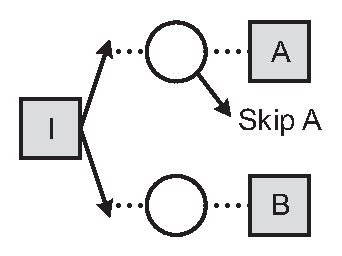
\includegraphics[width=0.27\textwidth]{fig_concurrent_case_a_1.eps}%
		\hspace{0.5in}%
		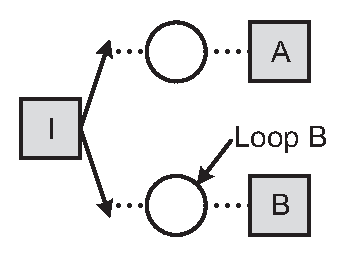
\includegraphics[width=0.27\textwidth]{fig_concurrent_case_a_2.eps}
	\end{minipage}
	\label{fig:concurrentCaseA}
}
\subfigure[] {
	\begin{minipage}[b]{0.45\textwidth}
		\centering
		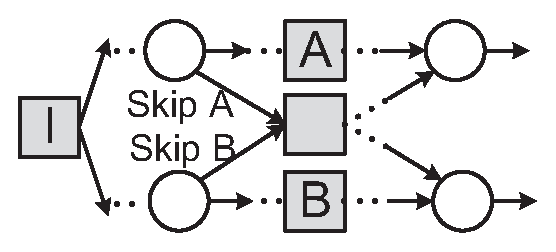
\includegraphics[width=0.7\textwidth]{fig_concurrent_case_b.eps}
	\end{minipage}
	\label{fig:concurrentCaseB}
}
\subfigure[] {
	\begin{minipage}[b]{0.45\textwidth}
		\centering
		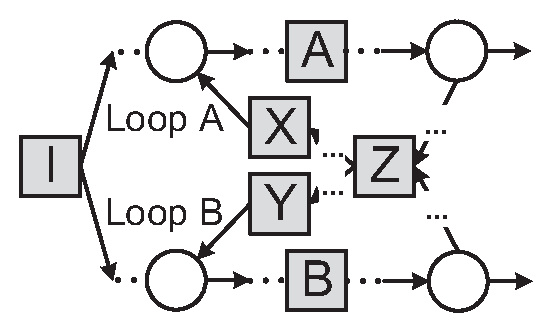
\includegraphics[width=0.7\textwidth]{fig_concurrent_case_c.eps}
	\end{minipage}
	\label{fig:concurrentCaseC}
}
\subfigure[] {
	\begin{minipage}[b]{0.45\textwidth}
		\centering
		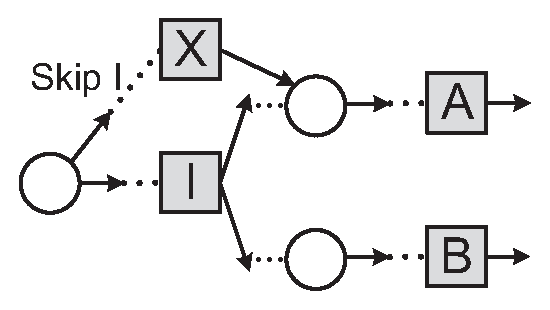
\includegraphics[width=0.7\textwidth]{fig_concurrent_case_d.eps}
	\end{minipage}
	\label{fig:concurrentCaseD}
}
\caption{Abstract formulas of concurrent relations. \subref{fig:concurrentCaseA} $A\Uparrow B$; \subref{fig:concurrentCaseB} $A\equiv B$; \subref{fig:concurrentCaseC} $A\equiv B$; \subref{fig:concurrentCaseD} $A\Uparrow B$.}
\label{fig:concurrentCases}
\end{figure}

Similarly as the abstract formulas for causal and inverse causal relations, we use symbol $*$ to represent any numbers of sequential events besides $A$ and $B$. In Fig. \ref{fig:concurrentCaseA}, we have traces such as $[I*A*B*],[I*B*A*],[I*A*]$ for the first unfolding and traces such as $[I*A*B*],[I*A*A*B*],[I*A*A*A*B*]...$ for the second unfolding, which do not satisfy the second condition in Definition \ref{def:alwaysConcurrent}. Therefore, events $A$ and $B$ of the unfoldings in Fig. \ref{fig:concurrentCaseA} are in \textit{sometimes concurrent} relation.

As for the unfolding in Fig. \ref{fig:concurrentCaseB}, events $A$ and $B$ may be executed both once or not executed at all, i.e., there are traces such as $[I*A*B*],[I*B*A*],[I*X*]$, indicating that $A\equiv B$. It is easily seen that traces in the unfolding of Fig. \ref{fig:concurrentCaseC} satisfy the second rule in Definition \ref{def:alwaysConcurrent}, so $A$ and $B$ are in \textit{always concurrent} relation. The unfolding in Fig. \ref{fig:concurrentCaseD} shows a special structure called non-free choice, and we will go into details later.

\subsection{Computing Extended Refined Ordering Relations Based on Unfolding}\label{subsec:computationOfRelations}
In Section \ref{subsec:causalAndInverseCausal} and Section \ref{subsec:concurrent}, we give the definitions of extended refined ordering relations with uncertainty between events of the complete prefix unfolding. 

As mentioned before, an intuitive idea to derive our relations is based on reachability graphs. Such technique would face a state explosion problem, especially when the WF-net contains a parallel with large scale of transitions. Theoretically, the reachability graph will derive all the reaching states by combining the executions of transitions within a parallel structure. Another problem is that we actually cannot distinguish the relation of \textit{response} and \textit{alternate response} in a WF-net with loop structure using the reachability technique. So we adopt the unfolding technology in this paper. The reason why we do not derive the relations based on sound WF-net itself is that WF-net describe the structure of a process rather than behaviors, which is just the focus of unfolding technique.

We may notice the fact that the computations of causal relation and inverse causal relation are similar in the way that we regard inverse causal relation as causal relation in the reversion of the unfolding. In another word, if we reverse the direction of every edge in the unfolding, then the causal relations in the new unfolding (actually the new graph is not an unfolding, but we use the saying to explain our computation here) are the same as the inverse causal relations in the original unfolding. This indicates that we can use the algorithm of causal relations to derive the inverse causal relations by backtracing nodes along the paths of an unfolding. The algorithm to derive causal relations between events of an unfolding is shown in Algorithm \ref{algo:causalRelations}. 

\begin{algorithm}[htbp]
\caption{Derive Causal Relations Between Events}
\label{algo:causalRelations}
	\begin{algorithmic}
		\Require a complete prefix unfolding $\beta=(B,E,A,f)$ and two events $a,b\in E$
		\Ensure causal relations between $a$ and $b$
		\If {there is no path from $a$ to $b$}
			\State \Return $a\nrightarrow b$
		\EndIf
		\State $path\gets$ some path from $a$ to $b$
		\If {$a==b$}
			\State \Return $a\rightharpoonup b$
		\Else
			\For {each condition $c\in path$}
				\State $Corr_{C}(c)\gets$ the set containing all the corresponding conditions of $c$
				\For {each $co\in Corr_{C}(c)$}
					\State $e\gets$ the succession event of $co$
					\If {there is a path from $e$ to $a$ or sink state without $b$}
						\State \Return $a\rightharpoonup b$
					\EndIf
				\EndFor
			\EndFor
		\EndIf
		\State \Return $a\twoheadrightarrow b$
	\end{algorithmic}
\end{algorithm}

As for the extended concurrent relations between events $a$ and $b$, there are actually two relations which should be taken into consideration, i.e., $a\parallel b$ and $b\parallel a$. We give the computation of such relations in Algorithm \ref{algo:concurrentRelations}.

\begin{algorithm}[htbp]
\caption{Derive Concurrent Relations Between Events}
\label{algo:concurrentRelations}
	\begin{algorithmic}
	\Require a complete prefix unfolding $\beta=(B,E,A,f)$, two events $a,b\in E$ and their least common predecessor $lcp$
	\Ensure concurrent relations between $a$ and $b$
	\If {$lcp$ is a condition OR $lcp==a$ OR $lcp==b$}
		\State \Return $a\nparallel b,b\nparallel a$
	\EndIf
	\State $path1\gets$ some path from $lcp$ to $a$
	\State $path2\gets$ some path from $lcp$ to $b$
	\State $aSkipSplits,bSkipSplits,aSkipJoins,bSkipJoins\gets\emptyset$
	\For {each condition $c\in path1$}
		\State $Corr_{C}(c)\gets$ the set containing all the corresponding conditions of $c$
		\For {each $co\in Corr_{C}(c)$}
			\State $se\gets$ the successive event of $co$
			\If {$se\notin path1$ AND there is a path from $se$ to sink state}
				\State $aSkipSplits\gets aSkipSplits\cup\{se\}$
			\EndIf
			\State $pe\gets$ the predecessive event of $co$
			\If {$pe\notin path1$ AND ($a==pe$ OR there is a path from source state or $a$ to $pe$ without any nodes of $path1$)}
				\State $aSkipJoins\gets aSkipJoins\cup\{pe\}$
			\EndIf
		\EndFor
	\EndFor
	\State Derive the set $bSkipSplits$ and $bSkipJoins$ by $path2$ using the method above
	\State $aSometimesConcurrent\gets\texttt{false},bSometimesConcurrent\gets\texttt{false}$
	\For {each event $aSucc\in aSkipSplits$}
		\For {each event $bSucc\in bSkipSplits$}
			\If {$aSucc==bSucc$}
				\State remove $aSucc$ from $aSkipSplits$ and remove $bSucc$ from $bSkipSplits$
			\EndIf
		\EndFor
	\EndFor
	\For {each event $aPred\in aSkipJoins$}
		\For {each event $bPred\in bSkipJoins$}
			\State $\_lcp\gets$ the lease common predecessor node of $aPred$ and $bPred$
			\If {$\_lcp$ is an event AND $\_lcp\neq lcp$}
				\State remove $bPred$ from $bSkipJoins$ and remove $bPred$ from $bSkipJoins$
			\EndIf
		\EndFor
	\EndFor
	\If {$aSkipSplits=\emptyset$ AND $aSkipJoins=\emptyset$}
		\If {$bSkipSplits=\emptyset$ AND $bSkipJoins=\emptyset$}
			\State \Return $a\equiv b,b\equiv a$
		\Else 
			\State \Return $a\equiv b,b\Uparrow a$
		\EndIf
	\Else
		\If {$bSkipSplits=\emptyset$ AND $bSkipJoins=\emptyset$}
			\State \Return $a\Uparrow b,b\equiv a$
		\Else 
			\State \Return $a\Uparrow b,b\Uparrow a$
		\EndIf
	\EndIf
	\end{algorithmic}
\end{algorithm}

More useful information are the extended relations between transitions on the WF-net, which can be utilized to check the consistency or measure the similarity between process models. , we focus on the computation of our relations on a WF-net based on its unfolding.

There may be more than one corresponding event (shadow event in some paper like \cite{wang2013efficient}) in the complete prefix unfolding of a transition in the original WF-net. These corresponding events are different from each other and are treated as unique events when we derive the relations between events in the unfolding. Therefore, when we try to derive the extended ordering relation between transitions in the WF-net, we need to check the relations between each corresponding event of those transitions. Based on this, we give the computation of extended relations between transitions. Let $Corr_{E}(A)$ be the set containing the corresponding events of transition $A$.

\begin{definition}[Extended Causal Relations Between Transitions]\label{def:causalRelations}
Transitions $A$ and $B$ are in
	\begin{itemize}
		\item[-] always causal relation (denoted as $A\twoheadrightarrow B$) iff: $\forall a\in Corr_{E}(A), \exists b\in Corr_{E}(B),\\s.t.~a\twoheadrightarrow b$;
		\item[-] never causal relation (denoted as $A\nrightarrow B$) iff: $\forall a\in Corr_{E}(A), b\in Corr_{E}(B),\\a\nrightarrow b$;
		\item[-] sometimes causal relation (denoted as $A\rightharpoonup B$) iff: $A$ and $B$ are neither in always causal relation nor in never causal relation.
	\end{itemize}
\end{definition}

\begin{definition}[Extended Inverse Causal Relations Between Transitions]\label{def:inverseCausalRelations}
Transitions $A$ and $B$ are in
	\begin{itemize}
		\item[-] always inverse causal relation (denoted as $B\twoheadrightarrow^{-1}A$) iff: $\forall b\in Corr_{E}(B), \exists a\in Corr_{E}(A), s.t.~b\twoheadrightarrow^{-1}a$;
		\item[-] never inverse causal relation (denoted as $B\nrightarrow^{-1}A$) iff: $\forall b\in Corr_{E}(B), a\in Corr_{E}(A), b\nrightarrow^{-1}a$;
		\item[-] sometimes inverse causal relation (denoted as $B\rightharpoonup^{-1}A$) iff: $A$ and $B$ are neither in always inverse causal relation nor in never inverse causal relation.
	\end{itemize}
\end{definition}

\begin{definition}[Extended Concurrent Relations Between Transitions]\label{def:concurrentRelations}
Transitions $A$ and $B$ are in
	\begin{itemize}
		\item[-] always concurrent relation (denoted as $A\equiv B$) iff: $\forall a\in Corr_{E}(A),\exists b\in Corr_{E}(B),s.t.~a\equiv b$;
		\item[-] never concurrent relation (denoted as $A\nparallel B$) iff: $\forall a\in Corr_{E}(A),b\in Corr_{E}(B),a\nparallel b$;
		\item[-] sometimes concurrent relation (denoted as $A\Uparrow B$) iff: $A$ and $B$ are neither in always concurrent relation nor in never concurrent relation.
	\end{itemize}
\end{definition}

Using the notions and computations described in the previous sections, we can derive the extended relations of the model in Fig. \ref{fig:examplePetri}. For convenience, we use a matrix to present three types of relations, as shown in Table \ref{tab:example_relations}. Transitions in the first column are the former ones in a relation while transitions in the first row are the latter ones in a relation. For example, the second row are the relations between $A$ and the other transitions. Due to limited space, we show three types of relations in one table cell. The rightmost table cell with relation symbols represents the relations between $A$ and $O$, i.e., $A\twoheadrightarrow O,A\nrightarrow^{-1}O,A\nparallel O$.

\begin{table}[htbp]
\caption{Extended relations of the model in Fig. \ref{fig:examplePetri}}
\label{tab:example_relations}
\centering
	\begin{tabular}{c|c|c|c|c|c|c|c} \hline
		Transitions & $A$ & $B$ & $C$ & $D$ & $E$ & $I$ & $O$\\ \hline
		$A$ 
			& \tabincell{c}{$\nrightarrow$\\$\nrightarrow^{-1}$\\$\nparallel$} 
			& \tabincell{c}{$\nrightarrow$\\$\nrightarrow^{-1}$\\$\nparallel$} 
			& \tabincell{c}{$\twoheadrightarrow$\\$\nrightarrow^{-1}$\\$\nparallel$} 
			& \tabincell{c}{$\nrightarrow$\\$\nrightarrow^{-1}$\\$\equiv$} 
			& \tabincell{c}{$\nrightarrow$\\$\nrightarrow^{-1}$\\$\Uparrow$} 
			& \tabincell{c}{$\nrightarrow$\\$\twoheadrightarrow^{-1}$\\$\nparallel$} 
			& \tabincell{c}{$\twoheadrightarrow$\\$\nrightarrow^{-1}$\\$\nparallel$}
			\\ \hline
		$B$ 
			& \tabincell{c}{$\nrightarrow$\\$\nrightarrow^{-1}$\\$\nparallel$} 
			& \tabincell{c}{$\nrightarrow$\\$\nrightarrow^{-1}$\\$\nparallel$} 
			& \tabincell{c}{$\twoheadrightarrow$\\$\nrightarrow^{-1}$\\$\nparallel$} 
			& \tabincell{c}{$\nrightarrow$\\$\nrightarrow^{-1}$\\$\equiv$} 
			& \tabincell{c}{$\nrightarrow$\\$\nrightarrow^{-1}$\\$\Uparrow$} 
			& \tabincell{c}{$\nrightarrow$\\$\twoheadrightarrow^{-1}$\\$\nparallel$} 
			& \tabincell{c}{$\twoheadrightarrow$\\$\nrightarrow^{-1}$\\$\nparallel$}
			\\ \hline
		$C$ 
			& \tabincell{c}{$\nrightarrow$\\$\rightharpoonup^{-1}$\\$\nparallel$} 
			& \tabincell{c}{$\nrightarrow$\\$\rightharpoonup^{-1}$\\$\nparallel$} 
			& \tabincell{c}{$\nrightarrow$\\$\nrightarrow^{-1}$\\$\nparallel$} 
			& \tabincell{c}{$\nrightarrow$\\$\nrightarrow^{-1}$\\$\equiv$} 
			& \tabincell{c}{$\nrightarrow$\\$\nrightarrow^{-1}$\\$\Uparrow$} 
			& \tabincell{c}{$\nrightarrow$\\$\twoheadrightarrow^{-1}$\\$\nparallel$} 
			& \tabincell{c}{$\twoheadrightarrow$\\$\nrightarrow^{-1}$\\$\nparallel$}
			\\ \hline
		$D$ 
			& \tabincell{c}{$\nrightarrow$\\$\nrightarrow^{-1}$\\$\Uparrow$} 
			& \tabincell{c}{$\nrightarrow$\\$\nrightarrow^{-1}$\\$\Uparrow$} 
			& \tabincell{c}{$\nrightarrow$\\$\nrightarrow^{-1}$\\$\Uparrow$} 
			& \tabincell{c}{$\rightharpoonup$\\$\rightharpoonup^{-1}$\\$\nparallel$} 
			& \tabincell{c}{$\rightharpoonup$\\$\rightharpoonup^{-1}$\\$\nparallel$} 
			& \tabincell{c}{$\nrightarrow$\\$\rightharpoonup^{-1}$\\$\nparallel$} 
			& \tabincell{c}{$\rightharpoonup$\\$\nrightarrow^{-1}$\\$\nparallel$}
			\\ \hline
		$E$ 
			& \tabincell{c}{$\nrightarrow$\\$\nrightarrow^{-1}$\\$\Uparrow$} 
			& \tabincell{c}{$\nrightarrow$\\$\nrightarrow^{-1}$\\$\Uparrow$} 
			& \tabincell{c}{$\nrightarrow$\\$\nrightarrow^{-1}$\\$\Uparrow$} 
			& \tabincell{c}{$\twoheadrightarrow$\\$\twoheadrightarrow^{-1}$\\$\nparallel$} 
			& \tabincell{c}{$\rightharpoonup$\\$\rightharpoonup^{-1}$\\$\nparallel$} 
			& \tabincell{c}{$\nrightarrow$\\$\rightharpoonup^{-1}$\\$\nparallel$} 
			& \tabincell{c}{$\rightharpoonup$\\$\nrightarrow^{-1}$\\$\nparallel$}
			\\ \hline
		$I$ 
			& \tabincell{c}{$\rightharpoonup$\\$\nrightarrow^{-1}$\\$\nparallel$} 
			& \tabincell{c}{$\rightharpoonup$\\$\nrightarrow^{-1}$\\$\nparallel$} 
			& \tabincell{c}{$\twoheadrightarrow$\\$\nrightarrow^{-1}$\\$\nparallel$} 
			& \tabincell{c}{$\twoheadrightarrow$\\$\nrightarrow^{-1}$\\$\nparallel$} 
			& \tabincell{c}{$\rightharpoonup$\\$\nrightarrow^{-1}$\\$\parallel$} 
			& \tabincell{c}{$\nrightarrow$\\$\nrightarrow^{-1}$\\$\nparallel$} 
			& \tabincell{c}{$\twoheadrightarrow$\\$\nrightarrow^{-1}$\\$\nparallel$}
			\\ \hline
		$O$ 
			& \tabincell{c}{$\nrightarrow$\\$\rightharpoonup^{-1}$\\$\nparallel$} 
			& \tabincell{c}{$\nrightarrow$\\$\rightharpoonup^{-1}$\\$\nparallel$} 
			& \tabincell{c}{$\nrightarrow$\\$\twoheadrightarrow^{-1}$\\$\nparallel$} 
			& \tabincell{c}{$\nrightarrow$\\$\twoheadrightarrow^{-1}$\\$\nparallel$} 
			& \tabincell{c}{$\nrightarrow$\\$\rightharpoonup^{-1}$\\$\nparallel$} 
			& \tabincell{c}{$\nrightarrow$\\$\twoheadrightarrow^{-1}$\\$\nparallel$} 
			& \tabincell{c}{$\twoheadrightarrow$\\$\nrightarrow^{-1}$\\$\nparallel$}
			\\ \hline
	\end{tabular}
\end{table}

\subsection{Sequential Direct Adjacency}\label{subsec:sda}
We can distinguish most process models from each other by their executing semantics using the extended refined ordering relations with uncertainty. However, there are still models with different semantics but the same extended relations, especially when invisible tasks are introduced. Invisible tasks do not appear in any log trace \cite{de2003workflow} . For more details about invisible tasks and their mining, please refer to the work of Wen \cite{wen2007mining}. 

\begin{figure}[h]
\centering
\subfigure[] {
	\centering
	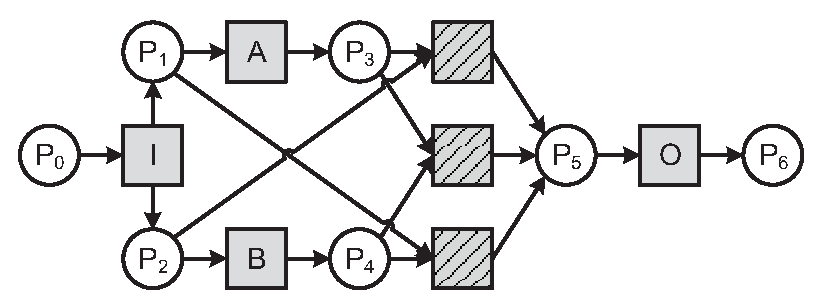
\includegraphics[width=0.45\textwidth]{fig_sda_example_1.eps}
	\label{fig:sdaExampleA}
}
\hspace{0.5cm}
\subfigure[] {
	\centering
	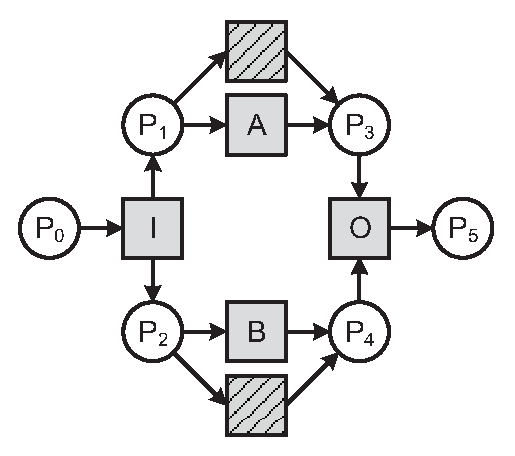
\includegraphics[width=0.45\textwidth]{fig_sda_example_2.eps}
	\label{fig:sdaExampleB}
}
\caption{Models with invisible tasks}
\label{fig:sdaExample}
\end{figure}

Fig. \ref{fig:sdaExample} shows an example. The full firing sequences of the model in Fig. \ref{fig:sdaExampleA} are $[I,A,B,O]$, $[I,B,A,O]$, $[I,A,O]$ and $[I,B,O]$ while the full firing sequences of the model in Fig. \ref{fig:sdaExampleB} are $[I,A,B,O]$, $[I,B,A,O]$, $[I,A,O]$, $[I,B,O]$ and $[I,O]$. But the extended relations of these two models are the same, as shown in Table \ref{tab:sdaExample}.

\begin{table}[htbp]
\centering
\tabcaption{Extend relations of the models in Fig. \ref{fig:sdaExample}}
\label{tab:sdaExample}
\begin{tabular}{c|c|c|c|c} \hline
	Transitions & $A$ & $B$ & $I$ & $O$\\ \hline
	$A$
		& \tabincell{c}{$\nrightarrow$\\$\nrightarrow^{-1}$\\$\nparallel$} 
		& \tabincell{c}{$\nrightarrow$\\$\nrightarrow^{-1}$\\$\Uparrow$} 
		& \tabincell{c}{$\nrightarrow$\\$\twoheadrightarrow^{-1}$\\$\nparallel$} 
		& \tabincell{c}{$\twoheadrightarrow$\\$\nrightarrow^{-1}$\\$\nparallel$} 
		\\ \hline
	$B$
		& \tabincell{c}{$\nrightarrow$\\$\nrightarrow^{-1}$\\$\Uparrow$} 
		& \tabincell{c}{$\nrightarrow$\\$\nrightarrow^{-1}$\\$\nparallel$} 
		& \tabincell{c}{$\nrightarrow$\\$\twoheadrightarrow^{-1}$\\$\nparallel$} 
		& \tabincell{c}{$\twoheadrightarrow$\\$\nrightarrow^{-1}$\\$\nparallel$} 
		\\ \hline
	$I$
		& \tabincell{c}{$\rightharpoonup$\\$\nrightarrow^{-1}$\\$\nparallel$} 
		& \tabincell{c}{$\rightharpoonup$\\$\nrightarrow^{-1}$\\$\nparallel$} 
		& \tabincell{c}{$\nrightarrow$\\$\nrightarrow^{-1}$\\$\nparallel$} 
		& \tabincell{c}{$\twoheadrightarrow$\\$\nrightarrow^{-1}$\\$\nparallel$} 
		\\ \hline
	$O$
		& \tabincell{c}{$\nrightarrow$\\$\rightharpoonup^{-1}$\\$\nparallel$} 
		& \tabincell{c}{$\nrightarrow$\\$\rightharpoonup^{-1}$\\$\nparallel$} 
		& \tabincell{c}{$\nrightarrow$\\$\twoheadrightarrow^{-1}$\\$\nparallel$} 
		& \tabincell{c}{$\nrightarrow$\\$\nrightarrow^{-1}$\\$\nparallel$} 
		\\ \hline
\end{tabular}
\end{table}

By looking into the executing semantics of these models, we find that the introduction of invisible tasks influences the adjacency of transitions, i.e., $I$ can be directly followed by $O$ in Fig. \ref{fig:sdaExampleA}, but not in Fig. \ref{fig:sdaExampleB}. Inspired by the idea of TAR \cite{zha2010workflow}, we propose the concept of sequential direct adjacency to solve the problem of invisible task.

\begin{definition}[Sequential Direct Adjacency]\label{def:sda}
Let $\Sigma=(P,T,F,M_{0})$ be a WF-net and $A,B\in T$ are two visible transitions. $A$ and $B$ are in sequential direct adjacency iff:
	\begin{itemize}
		\item[-] $A$ and $B$ are not in cocurrency relation;
		\item[-] $\exists\sigma=[t_{1}t_{2}...t_{n}]\in\Omega,1\leq i<j\leq n,t_{i}=A,t_{j}=B,s.t.~\forall k\in(i,j),t_{k}$ is an invisible transition.
	\end{itemize}
$A\rightarrow_{D}B$ ("D" for \textit{direct}) if they are in sequential direct adjacency while $A\rightarrow_{I}B$ ("I" for \textit{indirect}) if not. The set of all the transition pair which are in sequential direct adjacency is the SDA-set of a model.
\end{definition}

We use sequential direct adjacency to distinguish those transition pair which can be executed adjacently from those which cannot. By applying Definition \ref{def:sda} on the models in Fig. \ref{fig:sdaExample}, we derive the \textit{SDA-set} as followed:
\begin{displaymath}
	\begin{aligned}
		&\text{(a)} A\rightarrow_{D}O, B\rightarrow_{D}O, I\rightarrow_{D}A, I\rightarrow_{D}B\\
		&\text{(b)} A\rightarrow_{D}O, B\rightarrow_{D}O, I\rightarrow_{D}A, I\rightarrow_{D}B, I\rightarrow_{D}O
	\end{aligned}
\end{displaymath}

Using the combination of extended refined ordering relations with uncertainty and sequential direct adjacency, we can distinguish the two models with invisible tasks as well as many model pairs from each other efficiently.

\section{Similarity Measure}\label{sec:similarity}
In this section, we give the computation of similarity value on two process models based on extended relations and sequential direct adjacency described in Section \ref{sec:relations}.

\subsection{The Importance of Relation}\label{subsec:importance}
When we measure the similarity between two models, we actually measure the similarity between the relations of them. But our extended relations cannot reflect the different possibilities of transitions that may fire in concurrent and exclusive structures. Motivated by the work of TAR++ \cite{wang2015tar++}, we bring in the concepts about the importance of relation.

\cite{wang2015tar++} has given enough details about the concept of the weight of an edge as well as three rules to determine it. Also, the computation of weights of a WF-net can be found in this paper. We give the definition of the importance of relation based on the weight of an edge.

\begin{definition}[The Importance of Relation]\label{def:importance}
Given a weighted WF-net $\Sigma$, for any ordered transition pair $A,B$ in an extended relation, we select one out-edge of $A$ and one in-edge of $B$, whose coefficients are $\alpha,\beta$ respectively.\\
We use the minimum number of $\alpha$ and $\beta$ as the importance value of the extended relation, i.e., $\min\{\alpha,\beta\}$.
\end{definition}

\subsection{Computation}\label{subsec:computation}
By combining extended relations, sequential direct adjacency and the importance of relation together, we give the computation of similarity value between two WF-nets. For any ordered transition pair $A,B$, we use a triple $R(A,B)=(\gamma,\delta,\theta)$ to represent their extended relation, where $\gamma$ is the uncertainty ("A" for \textit{always}, "S" for \textit{sometimes} and "N" for \textit{never}), $\delta$ is the sequential direct adjacency ("D" for \textit{direct} and "I" for \textit{indirect}), $\theta$ is the importance (between $0$ and $1$). For convenience, we use $R_{pair}$ to denote the transition pair of a relation $R$.

On the other hand, we think two extended relation with the same $\delta$ are more similar than two extended relation with different $\delta$, so we set a weight $\lambda$ to measure the influence of sequential direct adjacency.

For two extended relations $R1=(\gamma_{1},\delta_{1},\theta_{1})$ and $R2=(\gamma_{2},\delta_{2},\theta_{2})$ where $R1_{pair}=R2_{pair}$, we have:
\begin{equation}\label{eq:relationOperations}
	\begin{aligned}
		R_{1}\cap R_{2}&=
			\begin{cases}
				0~R1_{pair}&	\gamma_{1}\neq\gamma_{2}\\
				\lambda\times\min\{\theta_{1},\theta_{2}\}~R1_{pair}&	\gamma_{1}=\gamma_{2}\wedge\delta_{1}\neq\delta_{2}\\
				\min\{\theta_{1},\theta_{2}\}~R1_{pair}&	\gamma_{1}=\gamma_{2}\wedge\delta_{1}=\delta_{2}
			\end{cases}\\
		R_{1}\cup R_{2}&=	\max\{\theta_{1},\theta_{2}\}~R1_{pair}
	\end{aligned}
\end{equation}

We derive three sets $ExRelSet(M)$ of extended relations of a model $M$, namely $ExRelSet_{\rightarrow}(M)$, $ExRelSet_{\rightarrow^{-1}}(M)$ and $ExRelSet_{\parallel}(M)$. Now we give the definition of intersection and union operation of these sets.

\begin{definition}[Intersection and Union Operation of Relation]\label{def:relSetOperations}
Given two extended relation sets $ExRelSet1$ and $ExRelSet2$, which contain $m$ and $n$ elements respectively. The relations in these sets are marked $R=(\gamma_{R},\delta_{R},\theta_{R})$, whose transition pair is denoted as $R_{pair}$. Then we have:
	\begin{equation}\label{eq:relSetOperations}
		\begin{aligned}
			ExRelSet1\Cap ExRelSet2=&\{\theta_{R}Ri_{pair}|\theta_{R}=\min\{\theta_{Ri},\theta_{Rj}\},Ri\in ExRelSet1,\\
			&\quad Rj\in ExRelSet2,Ri_{pair}=Rj_{pair}\}\}\\
			ExRelSet1\Cup ExRelSet2=&\{\theta_{R}Ri_{pair}|\theta_{R}=\max\{\theta_{Ri},\theta_{Rj}\},Ri\in ExRelSet1,\\
			&\quad Rj\in ExRelSet2,Ri_{pair}=Rj_{pair}\}\}\\
			&\cup\{\theta_{Ri}Ri_{pair}|Ri\in ExRelSet1\\
			&\qquad \wedge\nexists R_{j}\in ExRelSet2,s.t.~Ri_{pair}=Rj_{pair}\}\\
			&\cup\{\theta_{Rj}Rj_{pair}|Rj\in ExRelSet2\\
			&\qquad \wedge\nexists R_{i}\in ExRelSet1,s.t.~Ri_{pair}=Rj_{pair}\}
		\end{aligned}
	\end{equation}
\end{definition}

\section{Experiments}\label{sec:experiments}

\section{Conclusion}\label{sec:conclusion}


\bibliographystyle{plain}
\bibliography{ref}
\end{document}